\section{Model}

\subsection{general ideas}

\subsubsection{the crystal mesh}

The crystal is sampled and meshed into prisms

\begin{itemize}

    \begin{figure}[H]
      \centerline{
        \resizebox{0.45\textwidth} {!} {\includegraphics{graphics/delauny_3.png}}
      }
      \caption{extruded plane of triangles}
      \label{graphic:extruded_mesh}
    \end{figure}

  \item The crystal is seen as a 2D plane that gets sampled by a set of
    points.\label{label:meshSampling}

  \item Delauny triangulation is used to connect these points to a mesh of
    triangles.

  \item The triangles are extruded by a thickness to generate a slice of
    prisms. This slice gets duplicated several times to cover the whole
    crystal.

  \item The sample points can be distributed non-uniformly to increase
    spatial resolution in areas of interest.

\end{itemize}



\subsubsection{ray tracing}

\begin{itemize}

  \item \textbf{Image: 2D propagation of ray through triangle structure}

  \item To calculate the amplification of a single ray from a position $r$
    to a sampled point $r_0$, the ray is traced along its path through the
    prisms. The intersections with prism surfaces define line segments of a
    certain length. These segments are used for gain calculation.

  \item Starting from point $r$ inside a prism $p$, there are 5 possible
    intersection planes for the ray. One plane for the top and bottom
    surfaces and one for each of the 3 horizontal sides of $p$.

  \item Based on the intersection plane, the next prism is known due to a
    neighboring relation in the datastructure.  neighbor relation, that you
    store in a list.

  \item The intersection is calculated for each prism along the path, until
    $r_0$ is reached.
  
  \item For each intersection, its contribution to the ray's gain is calculated
    as a function of its length.

  \item \textit{(formula for gain calculation)}

\end{itemize}



\subsubsection{Reflections}

\begin{itemize}

  \item Depending on the material and coating, there are different
    reflectivities on the crystal's surfaces.

  \item A fast simulation allows to take reflecting rays into account and to
    estimate the impact of lateral lasing.

  \item Only reflections on upper and lower plane implemented until now.

\end{itemize}



\subsubsection{Monte Carlo simulation}
\label{label:monteCarlo}

\begin{itemize}

  \item \textit{integral is expressed by formula} \cite[Daniel's Thesis]{ASE2010}

  \item Monte Carlo simulation as a way to calculate the integral for the whole
    crystal.

  \item \textit{formula for the additive Monte Carlo}

\end{itemize}






